%==============================================================================
%  Standalone PREVIEW of the "DataSAIL baseline" poster block.
%  Does NOT touch lowrank_poster.tex — reuses the same palette + macros so the
%  block renders exactly as it would in Column 1 (~33 cm wide).
%  Compile:  pdflatex datasail_block_preview.tex
%==============================================================================
\documentclass{article}
\usepackage[paperwidth=35cm, paperheight=26cm, margin=1cm]{geometry}
\usepackage[T1]{fontenc}
\usepackage[utf8]{inputenc}
\usepackage{helvet}
\renewcommand{\familydefault}{\sfdefault}
\usepackage{amsmath, amssymb}
\usepackage{tikz}
\usepackage{pifont}
\usepackage{xcolor}
\usetikzlibrary{arrows.meta, positioning, calc}
\pagestyle{empty}

%---- palette (copied from lowrank_poster.tex) ------------------------------
\definecolor{maroon}{HTML}{7A0C00}
\definecolor{ink}{HTML}{14243B}
\definecolor{blue}{HTML}{2563EB}
\definecolor{soft}{HTML}{F3F0EC}
\definecolor{softblue}{HTML}{EAF1FE}
\definecolor{rulec}{HTML}{D9C7C2}
\color{ink}

%---- macros (copied from lowrank_poster.tex) -------------------------------
\newcommand{\pblock}[1]{%
  \par\vspace{1.6ex}%
  \begin{center}{\color{maroon}\bfseries\Large #1}\end{center}%
  \vspace{-1.0ex}{\color{rulec}\rule{\linewidth}{1.3pt}}\par\vspace{0.6ex}}
\newcommand{\callout}[2]{%
  \begin{center}\colorbox{#1}{\begin{minipage}{0.93\linewidth}\vspace{0.5ex}
  #2\vspace{0.5ex}\end{minipage}}\end{center}}

\begin{document}
% preview at the real Column-1 width (~33 cm) so proportions match the poster
\noindent\begin{minipage}{33cm}

\pblock{The baseline: DataSAIL}
{\large \textbf{DataSAIL}\ {\footnotesize(\emph{Data Splitting Against
Information Leakage})}\ is the standard leakage-aware splitter and our closest
baseline. It targets the \emph{same} cross-split similarity — but solves it
\textbf{exactly}:}
\vspace{0.5ex}
\begin{center}
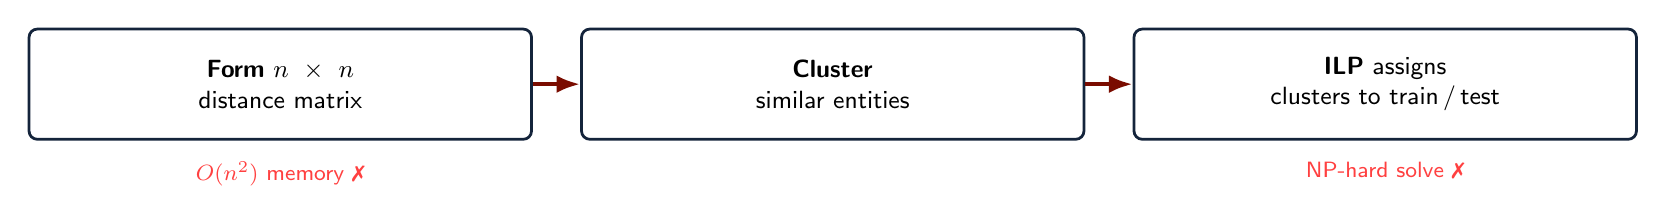
\begin{tikzpicture}[font=\small, node distance=6mm,
   b/.style={rectangle, rounded corners=3pt, draw=ink, line width=1pt,
     fill=white, align=center, inner sep=4pt, minimum height=14mm,
     text width=6.1cm},
   ar/.style={-{Latex[length=3mm]}, line width=1.5pt, draw=maroon}]
 \node[b] (d) {\textbf{Form} $n\times n$\\ distance matrix};
 \node[b, right=of d] (c) {\textbf{Cluster}\\ similar entities};
 \node[b, right=of c] (i) {\textbf{ILP} assigns\\ clusters to train\,/\,test};
 \draw[ar] (d)--(c); \draw[ar] (c)--(i);
 \node[red!75, below=1.5mm of d, font=\footnotesize] {$O(n^2)$ memory \ding{55}};
 \node[red!75, below=1.5mm of i, font=\footnotesize] {NP-hard solve \ding{55}};
\end{tikzpicture}
\end{center}
\vspace{0.3ex}
\callout{softblue}{\centering\large Faithful but \textbf{unscalable}: it must
\emph{materialize} the whole $n\times n$ similarity and solve a combinatorial
program — \textbf{90\,min} at 100k, \textbf{out-of-memory} by 300k.
\textbf{This is the gap we factorize away.}}

\end{minipage}
\end{document}
